\documentclass{beamer}
\usepackage{german}
\usepackage{graphicx}
\usepackage{tikz}
\usepackage{pgfplots}
\usepackage{xcolor}
\usepackage{eso-pic} %to draw on top right corner

%design & color
\usetheme{PaloAlto}
\usecolortheme{beaver}
\useinnertheme{circles}
\usefonttheme[onlymath]{serif}
\setbeamercolor{section in sidebar}{fg=black}
\setbeamercolor{itemize item}{fg=red}
\setbeamercolor{item projected}{fg=white,bg=black}

%disable navigation symbols
\beamertemplatenavigationsymbolsempty
%slide numbers
\setbeamertemplate{footline}[frame number]

%used for drawing n(r)-Area
\definecolor{lGray}{gray}{0.8}
\definecolor{llGray}{gray}{0.9}
\usepgfplotslibrary{fillbetween}
\usetikzlibrary{fadings}

\tikzset{
  ring shading/.code args={from #1 at #2 to #3 at #4}{
    \def\colin{#1}
    \def\radin{#2}
    \def\colout{#3}
    \def\radout{#4}
    \pgfmathsetmacro{\proportion}{\radin/\radout}
    \pgfmathsetmacro{\outer}{.8818cm}
    \pgfmathsetmacro{\inner}{.8818cm*\proportion}
    \pgfmathsetmacro{\innerlow}{\inner-0.01pt}
    \pgfdeclareradialshading{ring}{\pgfpoint{0cm}{0cm}}%
    {
      color(0pt)=(white);
      color(\innerlow)=(white);
      color(\inner)=(#1);
      color(\outer)=(#3)
    }
    \pgfkeysalso{/tikz/shading=ring}
  },
}


%texexternalize
\usetikzlibrary{external}
\usepgfplotslibrary{external} 
\tikzexternalize[] %prefix=tikz/
%\tikzset{external/mode=graphics if exists}

%use command const
\DeclareMathOperator{\const}{Konstant}

%title informations
\title[Licht] % (optional, only for long titles)
{Lichtbrechung an der Athmosphäre}
\author[Schaefer, Schneider] % (optional, for multiple authors)
{Simon Sch"afer \and Tibor Schneider}
\institute[hsr] % (optional)
{
  HSR Hochschule f"ur Technik Rapperswil
}
%\date[KPT 2004] % (optional)
%{Conference on Presentation Techniques, 2004}
\subject{Mathematik}

\begin{document}

  %titelseite
  \frame{\titlepage}  

  %inhaltsverzeichnis
  \frame{\frametitle{Inhaltsverzeichnis}\tableofcontents}
  
  \section{Einleitung}
  \begin{frame}
    \frametitle{Auswirkung der Lichtbrechung an der Athmosph"are}
    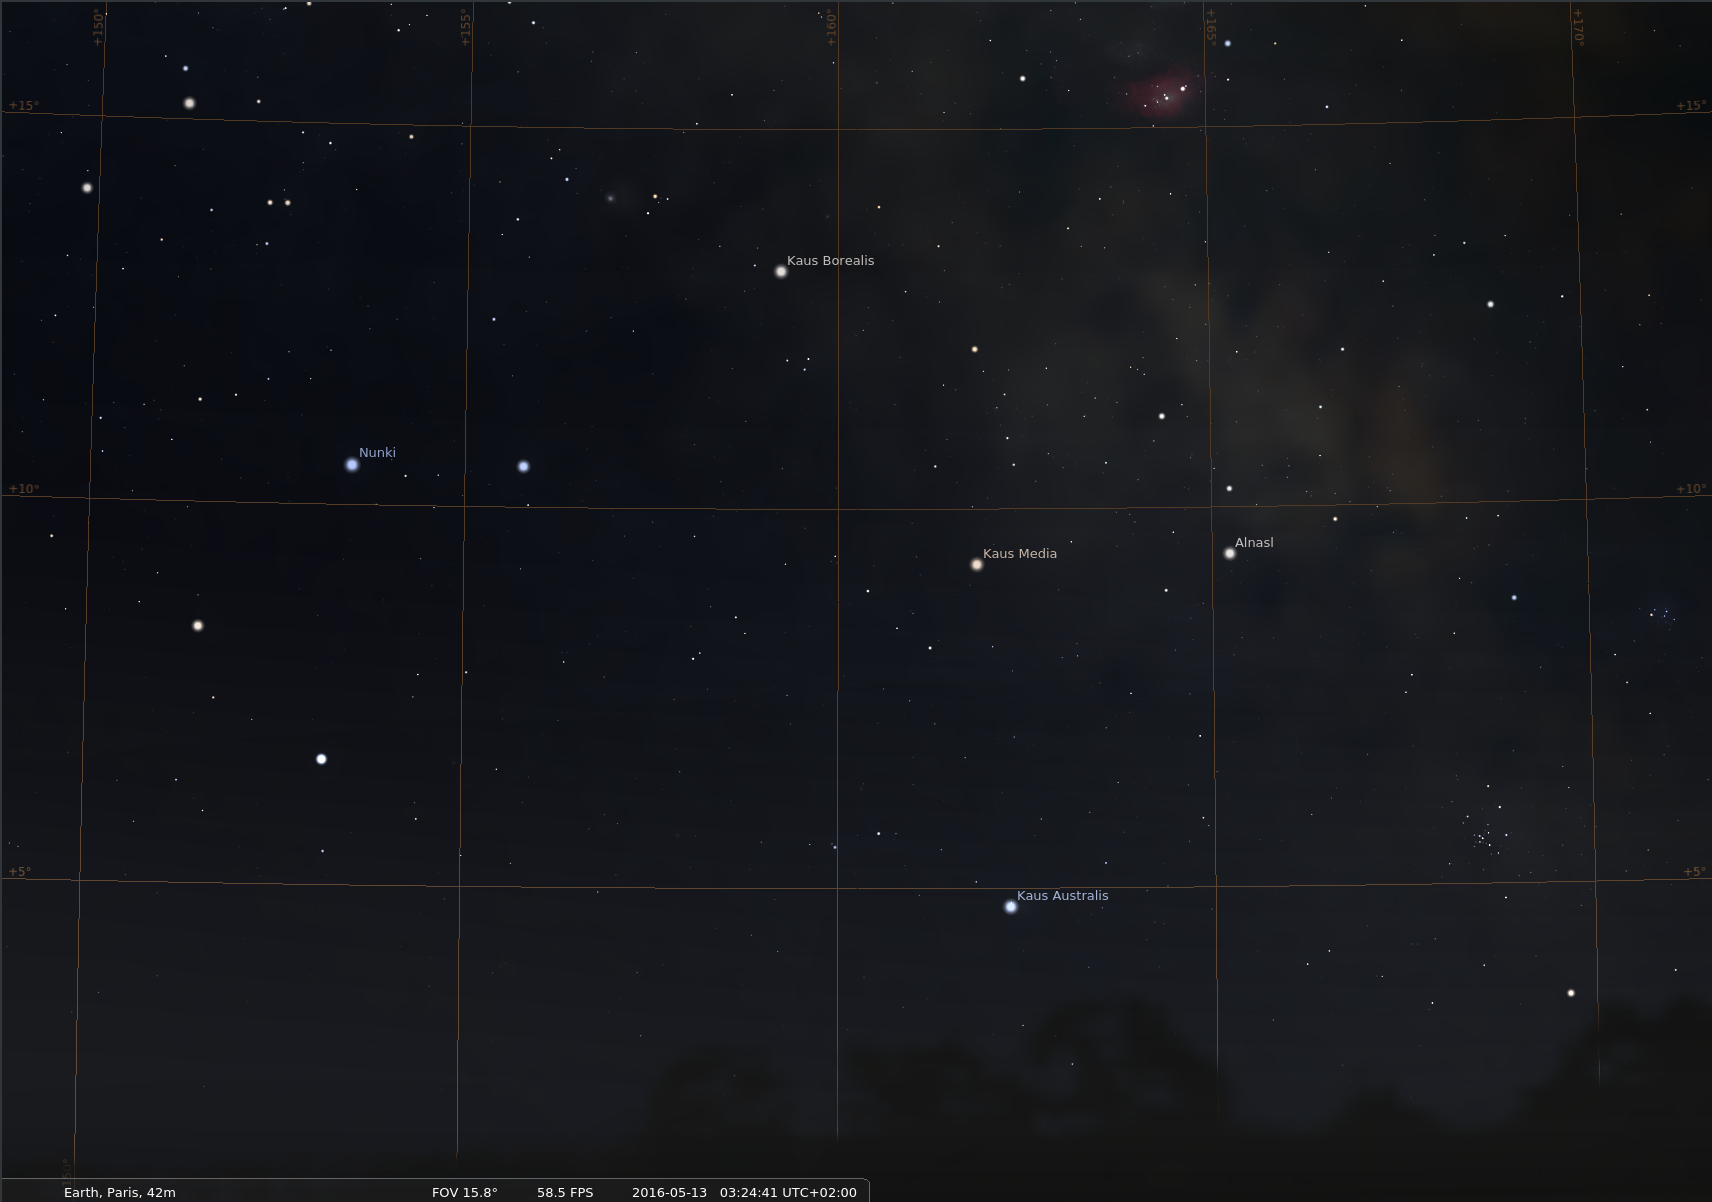
\includegraphics[width=\textwidth, trim={0 1cm 0 0}, clip]{images/stellarium_athmosphere}
  \end{frame} 
  \begin{frame}
    \frametitle{Auswirkung der Lichtbrechung an der Athmosph"are}
    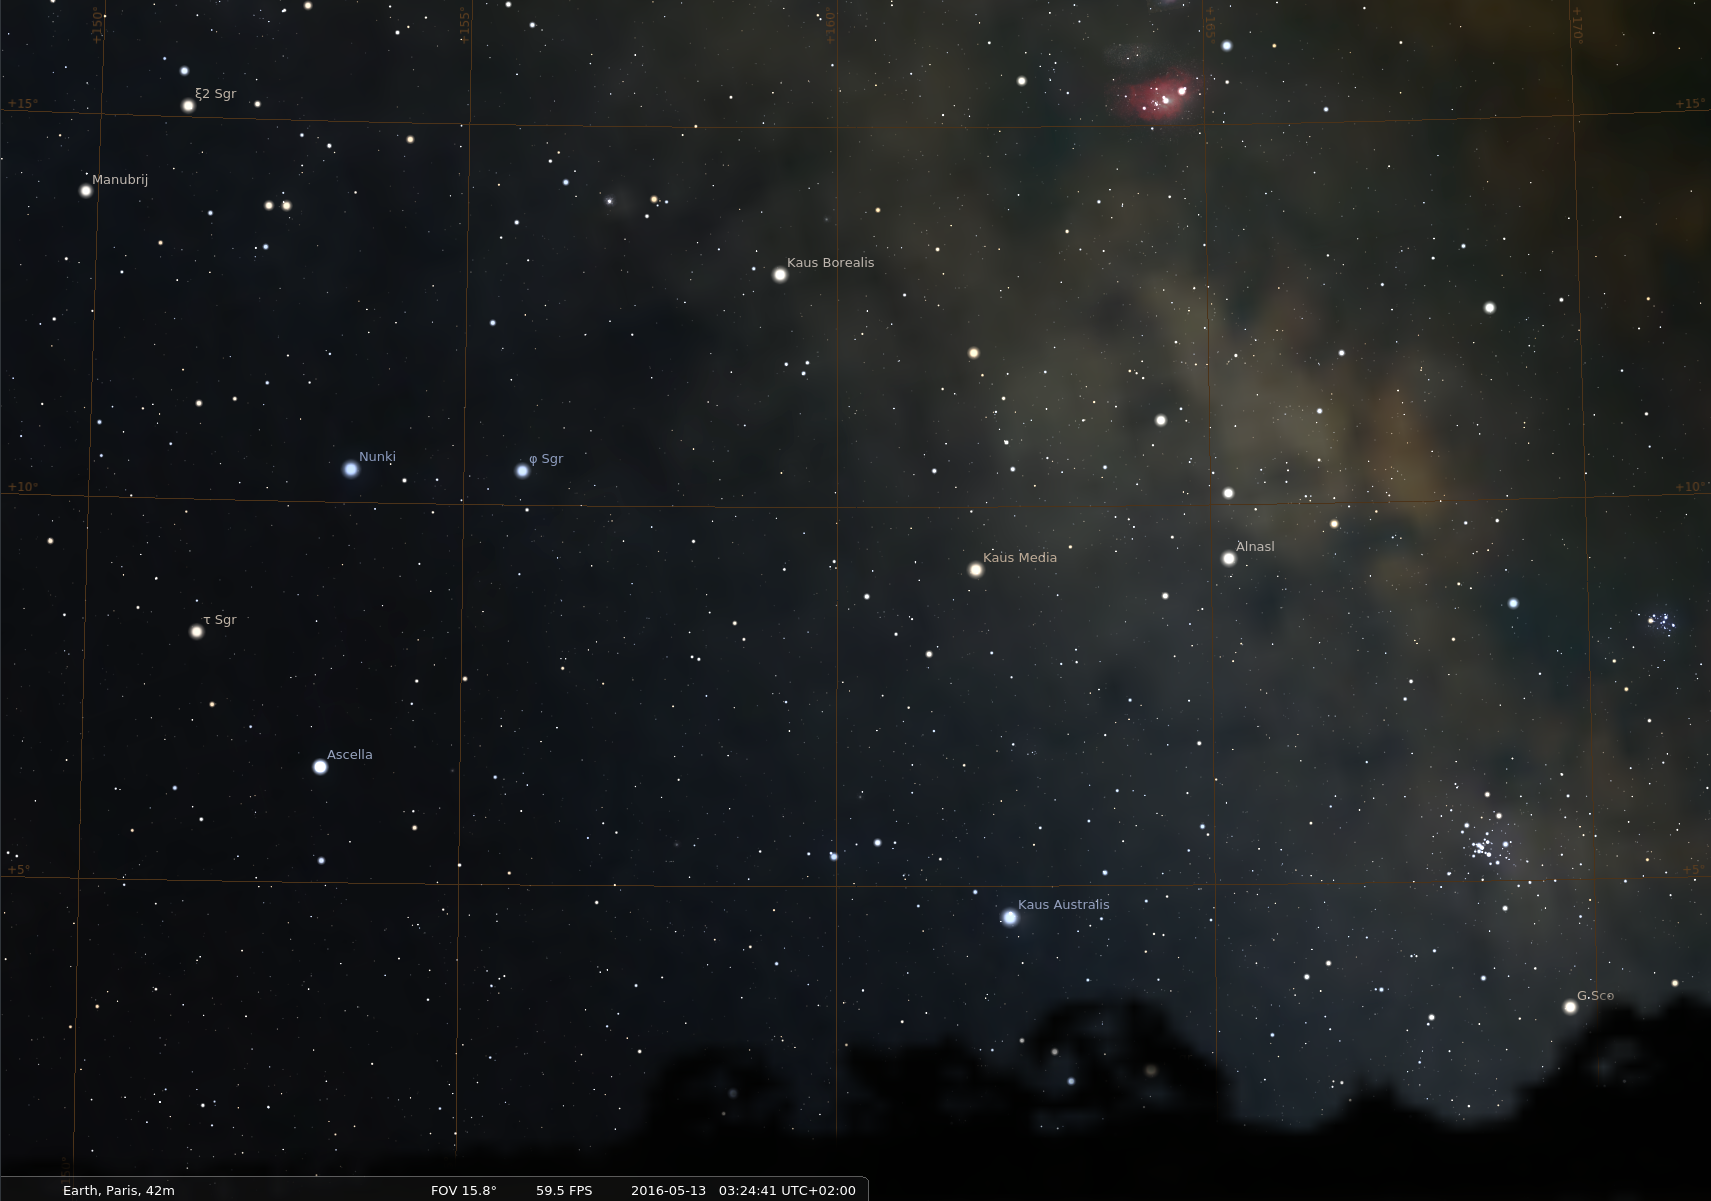
\includegraphics[width=\textwidth, trim={0 1cm 0 0}, clip]{images/stellarium_no_athmosphere}
  \end{frame} 
  
  \subsection{Snell's Law}
  \begin{frame}
    \frametitle{Snell's Law}

    \begin{center}
      \begin{tikzpicture}
        \draw [fill=llGray, draw=none] (0,0) rectangle (4,2);
        \draw (0,0) -- (4,0);
        \draw [dashed] (2,-2) -- (2,2);
        \draw (4,0.5) node [left] {$n_2$};
        \draw (4,-0.5) node [left] {$n_1$};
        \draw [thick, red] (0.5,-1.5) -- (2,0) -- (4,1.5);
        \draw (1.3,-0.7) arc (-135:-90:0.99) node [above left] {$\alpha_1$};
        \draw (2,0.99)  arc (90:36.8:0.99) node [left, yshift=+1mm, xshift=-1mm] {$\alpha_2$};
      \end{tikzpicture}
    \end{center} 
    
    $$\frac{n_1}{n_2} = \frac{\sin \alpha_2}{\sin \alpha_1}$$
    
    \begin{equation} \label{eq:snell}
      n_1 \cdot \sin \alpha_1 = n_2 \cdot \sin \alpha_2 
    \end{equation}
    
  \end{frame}

  \section{Planares Modell}
  \subsection{Herleitung}
  \begin{frame}
    \frametitle{Planares Modell}
    \framesubtitle{Herleitung (1)}
    
    \begin{center}
      \begin{tikzpicture}
        \begin{axis}[xlabel=$x$, ylabel = $y$, axis lines=middle, height=5cm, width = 8cm,
          ymin=0, ymax=1.5, xmin=0, xmax=1, yticklabels={$y_0$, $y$, $y + dy$}, ytick =
          {0.2,0.5,0.7}, xtick={0.2}, xticklabel={\rlap{$x_0$}}]
        
          \draw[dashed] (axis cs:0,0.5) -- (axis cs:1,0.5);
          \draw[dashed] (axis cs:0,0.7) -- (axis cs:1,0.7);
          \draw[dashed] (axis cs:0,0.5) -- (axis cs:1,0.5);
          \draw[dashed] (axis cs:0.2,0) -- (axis cs:0.2,0.2);
          \draw[dashed] (axis cs:0,0.2) -- (axis cs:0.2,0.2);
          \filldraw (axis cs:0.2,0.2) circle (2pt) node[anchor=north east] {$A$};
          \draw (axis cs:0.2,0.2) -- (axis cs:0.6,0.7);
          \draw (axis cs:0.6,0.7) -- (axis cs:1,1);
          \draw (axis cs:0.52, 0.595) arc (210:270:0.6cm) node[anchor=north east, yshift =
            +0.44cm] {$\alpha$};
          \draw (axis cs:0.688,0.762) arc (19:90:0.6cm) node[anchor=west, yshift=+0.05cm,
            xshift=+0.2cm] {$\alpha + d\alpha$};  
          \draw[dashed](axis cs:0.6,0.4) -- (axis cs:0.6,1);
           \draw (axis cs:0.3, 0.6) node {$n$};
          \draw (axis cs:0.3, 0.8) node {$n + dn$};
        \end{axis}
      \end{tikzpicture}    
    \end{center}

    $$\text{Snell's Law: } \quad n_1 \cdot \sin \alpha_1 = n_0 \cdot \sin \alpha_0$$ 
    $$\frac{\cos \alpha}{\sin \alpha} = \frac{dy}{dx} = y'(x) \quad \Rightarrow \quad \sin^2 \alpha = \frac{1}{y'^2(x)+1}$$   
    
  \end{frame}

  \begin{frame}
    \frametitle{Planares Modell}
    \framesubtitle{Herleitung (2)}

    $$n^2 \cdot \frac{1}{y'^2 + 1} = (n_0 \cdot \sin \alpha_0)^2$$  
        
    \begin{equation}
      y''(x) = \frac{n'_y}{n} \cdot \left( y'^2 + 1 \right) \qquad \text{mit } n'_y(y) = \frac{d n}{d y}
    \end{equation}  
    
  \end{frame}

  \subsection{Modellierung der Athmosph"are}
  \begin{frame}
    \frametitle{Modellierung der Athmosph"are}
    \framesubtitle{Erster Versuch: Verifikation}

    %display DGL in corner
    \AddToShipoutPictureFG*{
      \AtPageUpperLeft{
        \put(-5,-27){\makebox[\paperwidth][r]{$\displaystyle y''(x) = \frac{n'_y}{n} \cdot \left( y'^2 + 1 \right)$}}
      }
    }    
    
    $$n(y) = 1, \qquad n'_y = \frac{d n}{d y} = 0$$
    
    Einsetzen in die Differentialgleichung ergibt:
    
    $$y''(x) = 0$$ 
    $$y'(x) = y'(0)$$ 
    $$y(x) = y'(0) \cdot x + y(0)$$
    
  \end{frame}
  
  \begin{frame}
    \frametitle{Modellierung der Athmosph"are}
    \framesubtitle{Zweiter Versuch}

    %display DGL in corner
    \AddToShipoutPictureFG*{
      \AtPageUpperLeft{
        \put(-5,-27){\makebox[\paperwidth][r]{$\displaystyle y''(x) = \frac{n'_y}{n} \cdot \left( y'^2 + 1 \right)$}}
      }
    }
    
    
    $$n(y) = 1 + \mu \cdot e^{-\sigma y} \qquad n'_y(y) = -\sigma \mu \cdot e^{-\sigma y}$$   
    
    \pause 

    $$\text{Bei dieser Simulation:} \quad \mu = 1 \quad \sigma = \frac{1}{2}$$

    \begin{center}
      \begin{tikzpicture}
        \begin{axis}[xlabel=$x$, ylabel=$y(x)$, axis lines=middle, height=5cm, width=5cm, ticks
        = none, legend style={at={(1.1,0.5)}, anchor=west, draw=none},  ymin = 0, ymax = 10,
        xmin = 0, xmax = 10, colormap={traditionalpm3d}{color=(white) color=(lGray)}, %colorbar,
        view={0}{90}] 

        \addplot3[surf, domain=-10:10, y domain=0:20 , shader=flat, samples=61, forget plot] {1 + 1 * exp(-y/2)};  
        %\addlegendentry{$n(y)$}
  
        \addplot [mark = none, thick, draw=blue] coordinates{
        (0.00000,0.00000)(0.00008,0.00005)(0.00017,0.00010)(0.00025,0.00015)
        (0.00033,0.00020)(0.00075,0.00045)(0.00117,0.00070)(0.00159,0.00095)
        (0.00201,0.00121)(0.00410,0.00246)(0.00620,0.00371)(0.00829,0.00496)
        (0.01038,0.00622)(0.02085,0.01245)(0.03131,0.01866)(0.04178,0.02485)
        (0.05225,0.03100)(0.10458,0.06137)(0.15691,0.09107)(0.20924,0.12012)
        (0.26157,0.14852)(0.51157,0.27569)(0.76157,0.38962)(1.01157,0.49129)
        (1.26157,0.58151)(1.51157,0.66092)(1.76157,0.73009)(2.01157,0.78945)
        (2.26157,0.83938)(2.51157,0.88018)(2.76157,0.91208)(3.01157,0.93526)
        (3.26157,0.94986)(3.51157,0.95594)(3.76157,0.95354)(4.01157,0.94265)
        (4.26157,0.92322)(4.51157,0.89512)(4.76157,0.85822)(5.01157,0.81229)
        (5.26157,0.75706)(5.51157,0.69221)(5.76157,0.61731)(6.01157,0.53186)
        (6.26157,0.43525)(6.51157,0.32674)(6.76157,0.20546)(7.01157,0.07031)
        (7.26157,-0.08007)(7.51157,-0.24736)(7.76157,-0.43357)(8.01157,-0.64143)
        (8.26157,-0.87451)(8.51157,-1.13773)(8.76157,-1.43704)(9.01157,-1.78220)
        (9.26157,-2.18838)(9.40485,-2.45726)(9.54812,-2.76003)(9.69140,-3.10717)
        (9.83468,-3.51505)(9.87601,-3.64716)(9.91734,-3.78722)(9.95867,-3.93632)
        (10.00000,-4.09576)};
        \addlegendentry{$f'(0) = 0.6$}
    
        \addplot [mark = none, thick, draw=red] coordinates{
        (0.00000,0.00000)(0.00005,0.00005)(0.00010,0.00010)(0.00015,0.00015)
        (0.00020,0.00020)(0.00045,0.00045)(0.00070,0.00070)(0.00095,0.00095)
        (0.00121,0.00121)(0.00246,0.00246)(0.00372,0.00372)(0.00497,0.00497)
        (0.00623,0.00622)(0.01251,0.01248)(0.01879,0.01872)(0.02507,0.02495)
        (0.03135,0.03117)(0.06275,0.06202)(0.09415,0.09252)(0.12554,0.12267)
        (0.15694,0.15248)(0.31394,0.29668)(0.47093,0.43331)(0.62792,0.56302)
        (0.78491,0.68641)(1.03491,0.87100)(1.28491,1.04240)(1.53491,1.20197)
        (1.78491,1.35087)(2.03491,1.49003)(2.28491,1.62024)(2.53491,1.74218)
        (2.78491,1.85645)(3.03491,1.96356)(3.28491,2.06393)(3.53491,2.15797)
        (3.78491,2.24601)(4.03491,2.32835)(4.28491,2.40526)(4.53491,2.47697)
        (4.78491,2.54370)(5.03491,2.60563)(5.28491,2.66293)(5.53491,2.71574)
        (5.78491,2.76420)(6.03491,2.80844)(6.28491,2.84854)(6.53491,2.88461)
        (6.78491,2.91672)(7.03491,2.94495)(7.28491,2.96936)(7.53491,2.98999)
        (7.78491,3.00690)(8.03491,3.02011)(8.28491,3.02966)(8.53491,3.03557)
        (8.78491,3.03784)(9.03491,3.03648)(9.28491,3.03149)(9.53491,3.02286)
        (9.78491,3.01056)(9.83869,3.00744)(9.89246,3.00414)(9.94623,3.00068)
        (10.00000,2.99704)};
        \addlegendentry{$f'(0) = 1$}
    
        \addplot [mark = none, thick, draw=green] coordinates{
       (0.00000,0.00000)(0.00004,0.00005)(0.00007,0.00010)(0.00011,0.00015)
       (0.00014,0.00020)(0.00032,0.00045)(0.00050,0.00070)(0.00068,0.00095)
       (0.00086,0.00121)(0.00176,0.00246)(0.00266,0.00372)(0.00355,0.00497)
       (0.00445,0.00622)(0.00894,0.01249)(0.01342,0.01874)(0.01791,0.02498)
       (0.02239,0.03121)(0.04482,0.06220)(0.06725,0.09292)(0.08967,0.12337)
       (0.11210,0.15358)(0.22424,0.30091)(0.33638,0.44255)(0.44852,0.57900)
       (0.56065,0.71072)(0.81065,0.98925)(1.06065,1.24961)(1.31065,1.49459)
       (1.56065,1.72638)(1.81065,1.94668)(2.06065,2.15691)(2.31065,2.35825)
       (2.56065,2.55168)(2.81065,2.73803)(3.06065,2.91802)(3.31065,3.09225)
       (3.56065,3.26128)(3.81065,3.42555)(4.06065,3.58549)(4.31065,3.74145)
       (4.56065,3.89376)(4.81065,4.04271)(5.06065,4.18856)(5.31065,4.33154)
       (5.56065,4.47186)(5.81065,4.60971)(6.06065,4.74527)(6.31065,4.87869)
       (6.56065,5.01012)(6.81065,5.13969)(7.06065,5.26753)(7.31065,5.39374)
       (7.56065,5.51843)(7.81065,5.64170)(8.06065,5.76362)(8.31065,5.88429)
       (8.56065,6.00378)(8.81065,6.12216)(9.06065,6.23950)(9.31065,6.35585)
       (9.56065,6.47128)(9.67049,6.52171)(9.78033,6.57198)(9.89016,6.62209)
       (10.00000,6.67204) };
        \addlegendentry{$f'(0) = 1.4$}
    
        \addplot [mark = none, thick, draw=black] coordinates{
       (0.00000,0.00000)(0.00003,0.00005)(0.00006,0.00010)(0.00008,0.00015)
       (0.00011,0.00020)(0.00025,0.00045)(0.00039,0.00070)(0.00053,0.00095)
       (0.00067,0.00121)(0.00137,0.00246)(0.00207,0.00372)(0.00276,0.00497)
       (0.00346,0.00622)(0.00695,0.01249)(0.01044,0.01875)(0.01393,0.02499)
       (0.01742,0.03123)(0.03486,0.06227)(0.05230,0.09308)(0.06975,0.12366)
       (0.08719,0.15403)(0.17441,0.30265)(0.26163,0.44635)(0.34885,0.58556)
       (0.43606,0.72069)(0.64497,1.02972)(0.85387,1.32103)(1.06278,1.59761)
       (1.27168,1.86179)(1.52168,2.16416)(1.77168,2.45381)(2.02168,2.73271)
       (2.27168,3.00247)(2.52168,3.26436)(2.77168,3.51946)(3.02168,3.76864)
       (3.27168,4.01267)(3.52168,4.25218)(3.77168,4.48771)(4.02168,4.71973)
       (4.27168,4.94865)(4.52168,5.17481)(4.77168,5.39853)(5.02168,5.62008)
       (5.27168,5.83969)(5.52168,6.05756)(5.77168,6.27389)(6.02168,6.48883)
       (6.27168,6.70254)(6.52168,6.91513)(6.77168,7.12672)(7.02168,7.33741)
       (7.27168,7.54730)(7.52168,7.75647)(7.77168,7.96499)(8.02168,8.17292)
       (8.27168,8.38032)(8.52168,8.58724)(8.77168,8.79374)(9.02168,8.99986)
       (9.27168,9.20562)(9.45376,9.35529)(9.63584,9.50480)(9.81792,9.65416)
       (10.00000,9.80340) };
       \addlegendentry{$f'(0) = 1.8$}
    
  
        \end{axis}
      \end{tikzpicture}
    \end{center}    
    
  \end{frame}

  \subsection{Spezialfall}
  \begin{frame}
    \frametitle{Spezialfall: $y'(x) = 0$}
    
    Dieses Problem tritt an folgenden Stellen auf:
    \begin{itemize}
      \item \textbf{Geometrisch}: in $x$-Richtung "andert sich $n$ nicht.
      \item \textbf{In der Herleitung} wird durch $y'(x)$ geteilt.
    \end{itemize}
    
    Muss jedoch nicht behandelt werden weil:
    \begin{itemize}
      \item \textbf{In Realit"at}: Unregelm"assigkeiten in der Athmosph"are
      \item \textbf{Bei der Simulation}: wegen Quantisierungsfehler wird dieser Fall nie erreicht. 
    \end{itemize}
  \end{frame}  

  \section{Sph"arisches Modell}
  \subsection{Herleitung}
  \begin{frame}
    \frametitle{Sph"arisches Modell}
    \framesubtitle{Herleitung (1)}
    
    \begin{center}
      \begin{tikzpicture} [scale=0.7, transform shape]
        %radial lines
        \draw (0,0) node[above]{$O$} 
              -- ++(0:10cm)
              (0,0) -- ++(15:10cm)
              (0,0) -- ++(22.5:10cm);
        %Radius r0, r, r + dr      
        \draw ([shift=(-5:6cm)]0,0) arc (-5:27.5:6cm) node [above] {$r_0$}
              ([shift=(-4:8cm)]0,0) arc (-4:27.5:8cm) node [above] {$r$}
              ([shift=(-3.8:9cm)]0,0) arc (-3.8:27.5:9cm) node [above, xshift=-0.2cm] {$r +
              dr$};
        %path of the light
        \draw [thick] (0:6cm) node [above left]{A}
              -- (15:8cm) node [above left, yshift=-0.1cm] {$M$}
              -- (22.5:9cm) node [below right, yshift=0.1cm]{$N$}
              -- (28:9.5cm);
        \draw (22.5:8cm) node [above left, yshift=-0.1cm] {$H$};
        \draw (15:9cm) node[below right] {$P$};
        %angles
        \draw ([shift=(-157.5:0.8cm)]22.5:9cm) arc (-157.5:-113.2:0.8cm) node [above,
                yshift=0.1cm]{$\beta$}
              ([shift=(15:0.8cm)]15:8cm) arc (15:66.8:0.8cm) node [below,
                yshift = -0.15cm, xshift=0.1cm]{$\alpha$}
              ([shift=(22.5:0.6cm)]22.5:9cm) arc (22.5:85.9:0.6cm) node
                [xshift=0.7cm, yshift=0.2cm]{$\alpha+d\alpha$}
              ([shift=(0:0.8cm)]0:6cm) arc (0:50.2:0.8cm) node [below,
                yshift=-0.14cm]{$\alpha_0$}
              ([shift=(0:2.5cm)]0,0) arc (0:15:2.5cm) node [below left,
                yshift=-0.15cm]{$\varphi$}
              ([shift=(15:4.5cm)]0,0) arc (15:22.5:4.5cm) node [below left,
                yshift=-0.12cm]{$d\varphi$};
        %refraction rates
        \draw (10:6cm) node[fill=white] {$n_0$}
              (10:8cm) node[fill=white] {$n$}
              (10:9cm) node[fill=white] {$n + dn$};
        
      \end{tikzpicture}
    \end{center}

    $$\text{Snell's Law} \quad n \cdot \sin \beta = (n + dn) \cdot \sin (\alpha + d\alpha)$$
    $$\text{Dreieck OMN} \quad r \cdot \sin \alpha = (r + dr) \cdot \sin \beta$$
    \begin{equation} \label{eq:sphere_first}
      n r \sin \alpha = (n + dn)(r + dr) \sin(\alpha + d\alpha) = n_0 r_0 \sin \alpha_0   
    \end{equation} 
    
  \end{frame}    
  
  \begin{frame}
    \frametitle{Sph"arisches Modell}
    \framesubtitle{Herleitung (2)}
    
    \begin{center}
      \begin{tikzpicture} [scale=0.7, transform shape]
        %radial lines
        \draw (0,0) node[above]{$O$} 
              -- ++(0:10cm)
              (0,0) -- ++(15:10cm)
              (0,0) -- ++(22.5:10cm);
        %Radius r0, r, r + dr      
        \draw ([shift=(-5:6cm)]0,0) arc (-5:27.5:6cm) node [above] {$r_0$}
              ([shift=(-4:8cm)]0,0) arc (-4:27.5:8cm) node [above] {$r$}
              ([shift=(-3.8:9cm)]0,0) arc (-3.8:27.5:9cm) node [above, xshift=-0.2cm] {$r +
              dr$};
        %path of the light
        \draw [thick] (0:6cm) node [above left]{A}
              -- (15:8cm) node [above left, yshift=-0.1cm] {$M$}
              -- (22.5:9cm) node [below right, yshift=0.1cm]{$N$}
              -- (28:9.5cm);
        \draw (22.5:8cm) node [above left, yshift=-0.1cm] {$H$};
        \draw (15:9cm) node[below right] {$P$};
        %angles
        \draw ([shift=(-157.5:0.8cm)]22.5:9cm) arc (-157.5:-113.2:0.8cm) node [above,
                yshift=0.1cm]{$\beta$}
              ([shift=(15:0.8cm)]15:8cm) arc (15:66.8:0.8cm) node [below,
                yshift = -0.15cm, xshift=0.1cm]{$\alpha$}
              ([shift=(22.5:0.6cm)]22.5:9cm) arc (22.5:85.9:0.6cm) node
                [xshift=0.7cm, yshift=0.2cm]{$\alpha+d\alpha$}
              ([shift=(0:0.8cm)]0:6cm) arc (0:50.2:0.8cm) node [below,
                yshift=-0.14cm]{$\alpha_0$}
              ([shift=(0:2.5cm)]0,0) arc (0:15:2.5cm) node [below left,
                yshift=-0.15cm]{$\varphi$}
              ([shift=(15:4.5cm)]0,0) arc (15:22.5:4.5cm) node [below left,
                yshift=-0.12cm]{$d\varphi$};
        %refraction rates
        \draw (10:6cm) node[fill=white] {$n_0$}
              (10:8cm) node[fill=white] {$n$}
              (10:9cm) node[fill=white] {$n + dn$};
        
      \end{tikzpicture}
    \end{center}

    $$\text{Dreieck MNP} \quad \tan \alpha = \frac{\overline{NP}}{\overline{MP}} \quad \rightarrow \quad \sin^2 \alpha = \frac{1}{\left( \frac{r'}{r} \right)^2 + 1} $$    
    \begin{equation*}
      n r \sin \alpha = n_0 r_0 \sin \alpha_0 \tag{\ref{eq:sphere_first}}
    \end{equation*}
  \end{frame}
  
  \begin{frame}
    \frametitle{Sph"arisches Modell}
    \framesubtitle{Herleitung(3)}
    
    $$\frac{(n \cdot r)^2}{\left( \frac{r'}{r} \right)^2 + 1} = (r_0 n_0 \sin \alpha_0)^2$$
    \begin{equation} \label{eq:sphere_pre_ode}
      n'_r + n - \frac{nrr'' - nr'^2}{r'^2 + r^2} = 0
    \end{equation}
    \begin{equation} \label{eq:sphere_ode}
      r'' = \frac{n'_r r'^2 + n'_r r^2 + 2n r'^2 + nr^2}{n r} \qquad \text{mit } n'_r = \frac{d r}{d n}
    \end{equation}
  \end{frame}
  
  \begin{frame}
    \frametitle{Winkeldifferenz $\Delta \alpha$}

    \begin{center}
      \begin{tikzpicture}
        \draw [thick] (60:1) arc (60:120:1);
        \draw [blue, thick] plot [smooth] coordinates {(0.00000,1.00000)(-0.02913,1.01430)(-0.05912,1.02850)(-0.09001,1.04260)(-0.12186,1.05660)(-0.15622,1.07112)(-0.19174,1.08553)(-0.22848,1.09983)(-0.26652,1.11403)(-0.30594,1.12812)(-0.34683,1.14210)(-0.38928,1.15598)(-0.43341,1.16975)(-0.47931,1.18342)(-0.52714,1.19699)(-0.57702,1.21047)(-0.62912,1.22384)(-0.68363,1.23713)(-0.74072,1.25033)(-0.80064,1.26345)(-0.86364,1.27649)(-0.93000,1.28947)(-1.00004,1.30239)(-1.07415,1.31527)(-1.15276,1.32813)(-1.23636,1.34098)(-1.32554,1.35386)(-1.42096,1.36679)(-1.52345,1.37982)(-1.63395,1.39301)(-1.75359,1.40640)(-1.88375,1.42009)(-2.02615,1.43419)(-2.18287,1.44884)(-2.35647,1.46418)(-2.55025,1.48045)(-2.76851,1.49798)(-3.02833,1.51805)};
        \draw [dashed] (0,1) -- ++(153.43:3);
        \draw [dashed] (-3.02833,1.51805) -- ++(-4.417:3);
        \draw (136.549:3.08) arc (153.43:175.583:1.7) node [above right, yshift=-0.5mm] 
          {$\Delta \alpha$}; 
      \end{tikzpicture}
    \end{center}    
    
  \end{frame}
  
  \subsection{Modellierung der Athmosph"are}
  \begin{frame}
    \frametitle{Modellierung}
    \framesubtitle{Erster Versuch: Verifikation}

    $$n(r) = 1 \qquad n'_r(r) = 0$$    

    \pause    
    
    %display DGL in corner
    \AddToShipoutPictureFG*{
      \AtPageUpperLeft{
        \put(-5,-27){\makebox[\paperwidth][r]{$\displaystyle r''(\varphi) = \frac{n'_r r'^2 + n'_r r^2 + 2n r'^2 + nr^2}{n r}$}}
      }
    }
        
    \begin{center}    
      \begin{tikzpicture}
        \begin{axis} [
          axis lines=none, 
          width=6cm, 
          axis equal,
          ticks = none, 
          legend style={at={(1.1,0.5)}, anchor=west, draw=none}, 
          ymin = 0,
          ymax = 4,
          xmin = -3, 
          xmax = 3, 
        ]
          %f'(0)=1
          \addplot [mark = none, thick, color=red] coordinates {
            (0,1)(-0.01703,1.01703)(-0.03467,1.03467)(-0.05294,1.05294)(-0.07191,1.07191)(-0.09252,1.09252)(-0.11401,1.11401)(-0.13644,1.13644)(-0.15989,1.15989)(-0.18445,1.18445)(-0.21021,1.21021)(-0.23729,1.23729)(-0.26581,1.26581)(-0.29589,1.29590)(-0.32770,1.32771)(-0.36141,1.36141)(-0.39722,1.39722)(-0.43534,1.43534)(-0.47605,1.47605)(-0.51964,1.51964)(-0.56645,1.56645)(-0.61690,1.61690)(-0.67144,1.67145)(-0.73066,1.73066)(-0.79520,1.79520)(-0.86588,1.86589)(-0.94365,1.94366)(-1.02970,2.02970)(-1.12549,2.12549)(-1.23286,2.23287)(-1.35406,2.35407)(-1.49207,2.49207)(-1.65081,2.65082)(-1.83549,2.83555)(-2.05283,3.05284)(-2.31283,3.31280)(-2.62991,3.62995)(-2.92055,3.92067)(-3.26854,4.26856)
          };
          \addlegendentry{$r'(0) = 1$};
          %f'(0) = 0.5
          \addplot [mark = none, thick, color=blue] coordinates {
            (0.00000,1.00000)(-0.01689,1.00844)(-0.03408,1.01704)(-0.05158,1.02579)(-0.06941,1.03471)(-0.09670,1.04835)(-0.12486,1.06243)(-0.15395,1.07697)(-0.18407,1.09203)(-0.21530,1.10765)(-0.24776,1.12388)(-0.28157,1.14078)(-0.31684,1.15842)(-0.35374,1.17687)(-0.39241,1.19621)(-0.43305,1.21652)(-0.47586,1.23793)(-0.52108,1.26054)(-0.56898,1.28449)(-0.61987,1.30993)(-0.67411,1.33706)(-0.73213,1.36607)(-0.79440,1.39720)(-0.86150,1.43075)(-0.93410,1.46705)(-1.01303,1.50652)(-1.09925,1.54963)(-1.19395,1.59698)(-1.29858,1.64929)(-1.41496,1.70750)(-1.54531,1.77267)(-1.69253,1.84627)(-1.86039,1.93020)(-2.05385,2.02698)(-2.27927,2.13965)(-2.54589,2.27292)(-2.86683,2.43344)(-3.17156,2.58589)
          };
          \addlegendentry{$r'(0) = 0.5$};
        
          %draw Earth
          \addplot [domain=-1:1, mark=none, black, samples=101, name path=earth, thick] {sqrt(1 - x^2)};
        \end{axis} 
      \end{tikzpicture}
    \end{center}
    
  \end{frame}
  
  \begin{frame}
    \frametitle{Modellierung}
    \framesubtitle{Zweiter Versuch}
    
    %display DGL in corner
    \AddToShipoutPictureFG*{
      \AtPageUpperLeft{
        \put(-5,-27){\makebox[\paperwidth][r]{$\displaystyle r''(\varphi) = \frac{n'_r r'^2 + n'_r r^2 + 2n r'^2 + nr^2}{n r}$}}
      }
    }

    $$n(r)=1 + \mu \cdot e^{-\sigma (r - r_0)} \qquad n'_r(r) = -\sigma \mu \cdot e^{-\sigma (r-r_0)}$$   
    \pause
    $$\text{Parameter:} \quad \mu = 1, \quad \sigma = 0.5, \quad r_0 = r(0) = 1$$

    \begin{center}
      \begin{tikzpicture}
        \begin{axis} [
          axis lines=none, 
          width=6cm, 
          axis equal,
          ticks = none,  
          legend style={at={(1.1,0.5)}, anchor=west, draw=none}, 
          ymin = 0,
          ymax = 4,
          xmin = -3, 
          xmax = 3, 
          zmin = 1,
          zmax = 2,
          %colorbar, 
          colormap={traditionalpm3d}{color=(white) color=(llGray) color=(lGray) color=(lGray)},
          view={0}{90}
        ]  
          \addplot3[surf, domain=-4:4, y domain=0:4, shader=flat, samples=61, forget plot] {1 + 1 * exp(-(sqrt(x^2+y^2)-1)/2)};  
          %\addlegendentry{$n(r)$};
          %f'(0)=0,2
          \addplot [mark = none, thick, color=blue] coordinates {
            (0.00000,1.00000)(-0.01332,1.00264)(-0.02671,1.00523)(-0.04019,1.00778)(-0.05374,1.01028)(-0.09766,1.01802)(-0.14254,1.02531)(-0.18851,1.03217)(-0.23567,1.03858)(-0.28418,1.04453)(-0.33419,1.05001)(-0.38587,1.05501)(-0.43940,1.05950)(-0.49500,1.06345)(-0.55289,1.06684)(-0.61334,1.06963)(-0.67664,1.07177)(-0.74314,1.07321)(-0.81322,1.07389)(-0.88734,1.07372)(-0.96600,1.07263)(-1.04982,1.07052)(-1.13952,1.06724)(-1.23592,1.06265)(-1.34006,1.05657)(-1.45317,1.04879)(-1.57672,1.03902)(-1.71256,1.02692)(-1.86302,1.01211)(-2.03105,0.99406)(-2.22032,0.97204)(-2.43583,0.94521)(-2.68435,0.91244)(-2.97519,0.87217)(-3.32034,0.82190)(-3.73947,0.75864)(-4.26247,0.67763)(-4.66896,0.61339)(-5.15258,0.53572)(-5.74058,0.44042)(-6.47383,0.32098)(-7.07070,0.22331)(-7.78451,0.10590)(-8.65695,-0.03780)(-9.75048,-0.21781)(-10.64136,-0.36457)(-11.70941,-0.54087)(-13.01771,-0.75678)(-14.66075,-1.02765)(-16.00049,-1.24854)(-17.60807,-1.51390)(-19.57873,-1.83911)(-22.05519,-2.24749)(-24.04608,-2.57581)(-26.42972,-2.96917)(-29.34303,-3.44988)(-32.99002,-4.05137)(-34.44359,-4.29116)(-36.03173,-4.55315)(-37.77414,-4.84060)(-39.69468,-5.15743)
          };
          \addlegendentry{$r'(0) = 0.2, \: \Delta \alpha \approx 20.6^\circ$};
          %f'(0)=0.5
          \addplot [mark = none, thick, color=red] coordinates {
            (0.00000,1.00000)(-0.02287,1.01133)(-0.04628,1.02273)(-0.07026,1.03420)(-0.09484,1.04575)(-0.13129,1.06249)(-0.16915,1.07944)(-0.20856,1.09662)(-0.24964,1.11404)(-0.29253,1.13176)(-0.33741,1.14978)(-0.38445,1.16816)(-0.43386,1.18693)(-0.48586,1.20614)(-0.54073,1.22583)(-0.59876,1.24607)(-0.66027,1.26690)(-0.72567,1.28841)(-0.79538,1.31068)(-0.86993,1.33379)(-0.94992,1.35785)(-1.03605,1.38301)(-1.12913,1.40939)(-1.23016,1.43719)(-1.34033,1.46661)(-1.46106,1.49793)(-1.59408,1.53143)(-1.74156,1.56753)(-1.90621,1.60674)(-2.09152,1.64973)(-2.30177,1.69721)(-2.54287,1.75035)(-2.82274,1.81070)(-3.15233,1.88043)(-3.54591,1.96187)(-4.02657,2.05985)(-4.62950,2.18150)(-5.10124,2.27585)(-5.66443,2.38767)(-6.35138,2.52357)
          };
          \addlegendentry{$r'(0) = 0.5, \: \Delta \alpha \approx 15.2^\circ$};
          %f'(0) = 1
          \addplot [mark = none, thick, color=green] coordinates {
            (0.00000,1.00000)(-0.02159,1.02144)(-0.04413,1.04355)(-0.06769,1.06635)(-0.09234,1.08990)(-0.11988,1.11587)(-0.14885,1.14283)(-0.17938,1.17085)(-0.21158,1.20002)(-0.24561,1.23044)(-0.28162,1.26222)(-0.31980,1.29548)(-0.36035,1.33036)(-0.40350,1.36702)(-0.44952,1.40562)(-0.49869,1.44638)(-0.55136,1.48951)(-0.60791,1.53528)(-0.66881,1.58400)(-0.73457,1.63602)(-0.80580,1.69175)(-0.88324,1.75168)(-0.96772,1.81638)(-1.06026,1.88654)(-1.16211,1.96301)(-1.27477,2.04682)(-1.40005,2.13916)(-1.54024,2.24163)(-1.69827,2.35624)(-1.87786,2.48554)(-2.08370,2.63268)(-2.32226,2.80216)(-2.60238,3.00014)(-2.93643,3.23523)(-3.34070,3.51823)(-3.84233,3.86838)(-4.48359,4.31531)(-4.95937,4.64639)(-5.52919,5.04235)(-6.22631,5.52657)(-7.10070,6.13397)(-7.94788,6.72246)(-8.99750,7.45079)(-10.34128,8.38345)(-12.12876,9.62479)
          }; 
          \addlegendentry{$r'(0) = 1, \: \Delta \alpha \approx 10.0^\circ$}; 
          %f'(0) = 1.5
          \addplot [mark = none, thick, color=black] coordinates {
            (0.00000,1.00000)(-0.01361,1.02708)(-0.02797,1.05537)(-0.04315,1.08496)(-0.05920,1.11595)(-0.07620,1.14845)(-0.09421,1.18258)(-0.11334,1.21846)(-0.13366,1.25625)(-0.15530,1.29610)(-0.17836,1.33821)(-0.20298,1.38278)(-0.22931,1.43004)(-0.25752,1.48025)(-0.28781,1.53371)(-0.32040,1.59077)(-0.35553,1.65182)(-0.39350,1.71730)(-0.43465,1.78774)(-0.47937,1.86375)(-0.52812,1.94605)(-0.58146,2.03548)(-0.64001,2.13305)(-0.70457,2.23995)(-0.77608,2.35768)(-0.85569,2.48804)(-0.94482,2.63321)(-1.04524,2.79599)(-1.15925,2.97998)(-1.28981,3.18983)(-1.44064,3.43132)(-1.61699,3.71275)(-1.82607,4.04553)
          };        
          \addlegendentry{$r'(0) = 1.5, \: \Delta \alpha \approx 5.5^\circ$};
          %draw Earth
          \addplot [domain=-1:1, mark=none, black, samples=101, name path=earth, thick] {sqrt(1 - x^2)};
        \end{axis}   
      \end{tikzpicture}
    \end{center}
    
  \end{frame}
  
  \begin{frame}
    \frametitle{Modellierung}
    \framesubtitle{Zweiter Versuch}
    
    %display DGL in corner
    \AddToShipoutPictureFG*{
      \AtPageUpperLeft{
        \put(-5,-27){\makebox[\paperwidth][r]{$\displaystyle r''(\varphi) = \frac{n'_r r'^2 + n'_r r^2 + 2n r'^2 + nr^2}{n r}$}}
      }
    }

    $$n(r)=1 + \mu \cdot e^{-\sigma (r - r_0)} \qquad n'_r(r) = -\sigma \mu \cdot e^{-\sigma (r-r_0)}$$    
    
    $$\text{Parameter:} \quad \mu = 1, \quad \sigma = 1, \quad r_0 = r(0) = 1$$

    \begin{center}
      \begin{tikzpicture}
        \begin{axis} [
          axis lines=none, 
          width=6cm, 
          axis equal,
          ticks = none,  
          legend style={at={(1.1,0.5)}, anchor=west, draw=none}, 
          ymin = 0,
          ymax = 4,
          xmin = -3, 
          xmax = 3, 
          zmin = 1,
          zmax = 2,
          %colorbar, 
          colormap={traditionalpm3d}{color=(white) color=(llGray) color=(lGray) color=(lGray) color=(lGray) color=(lGray)},
          view={0}{90}
        ]  
          \addplot3[surf, domain=-4:4, y domain=0:4, shader=flat, samples=81, forget plot] {1 + 1 * exp(-(sqrt(x^2+y^2)-1))};  
          %\addlegendentry{$n(r)$};
          %f'(0)=0,2
          \addplot [mark = none, thick, color=blue] coordinates {
            (0.00000,1.00000)(-0.01801,1.00352)(-0.03615,1.00689)(-0.05442,1.01012)(-0.07284,1.01321)(-0.11443,1.01957)(-0.15680,1.02520)(-0.19999,1.03007)(-0.24407,1.03417)(-0.28911,1.03749)(-0.33517,1.03999)(-0.38232,1.04165)(-0.43065,1.04243)(-0.48026,1.04231)(-0.53123,1.04124)(-0.58369,1.03918)(-0.63774,1.03607)(-0.69354,1.03186)(-0.75122,1.02649)(-0.81095,1.01989)(-0.87293,1.01197)(-0.93737,1.00264)(-1.00451,0.99180)(-1.07463,0.97932)(-1.14805,0.96508)(-1.22513,0.94892)(-1.30629,0.93066)(-1.39204,0.91009)(-1.48295,0.88697)(-1.57972,0.86101)(-1.68316,0.83188)(-1.79427,0.79918)(-1.91426,0.76242)(-2.04464,0.72103)(-2.18719,0.67425)(-2.34428,0.62119)(-2.51893,0.56071)(-2.71505,0.49133)(-2.93756,0.41105)(-3.19352,0.31729)(-3.49277,0.20641)(-3.68095,0.13615)(-3.88930,0.05800)(-4.12164,-0.02945)(-4.38284,-0.12803)
          };
          \addlegendentry{$r'(0) = 0.2, \: \Delta \alpha \approx 32.7^\circ$};
          
          %f'(0)=0.5
          \addplot [mark = none, thick, color=red] coordinates {
            (0.00000,1.00000)(-0.02913,1.01430)(-0.05912,1.02850)(-0.09001,1.04260)(-0.12186,1.05660)(-0.15622,1.07112)(-0.19174,1.08553)(-0.22848,1.09983)(-0.26652,1.11403)(-0.30594,1.12812)(-0.34683,1.14210)(-0.38928,1.15598)(-0.43341,1.16975)(-0.47931,1.18342)(-0.52714,1.19699)(-0.57702,1.21047)(-0.62912,1.22384)(-0.68363,1.23713)(-0.74072,1.25033)(-0.80064,1.26345)(-0.86364,1.27649)(-0.93000,1.28947)(-1.00004,1.30239)(-1.07415,1.31527)(-1.15276,1.32813)(-1.23636,1.34098)(-1.32554,1.35386)(-1.42096,1.36679)(-1.52345,1.37982)(-1.63395,1.39301)(-1.75359,1.40640)(-1.88375,1.42009)(-2.02615,1.43419)(-2.18287,1.44884)(-2.35647,1.46418)(-2.55025,1.48045)(-2.76851,1.49798)(-3.02833,1.51805)(-3.32895,1.54037)(-3.68221,1.56589)(-4.10493,1.59591)
          };
          \addlegendentry{$r'(0) = 0.5, \: \Delta \alpha \approx 22.1^\circ$};
          
          %f'(0) = 1
          \addplot [mark = none, thick, color=green] coordinates {
            (0.00000,1.00000)(-0.02171,1.02148)(-0.04437,1.04344)(-0.06804,1.06590)(-0.09278,1.08889)(-0.11864,1.11245)(-0.14571,1.13661)(-0.17405,1.16141)(-0.20374,1.18689)(-0.23488,1.21311)(-0.26756,1.24010)(-0.30190,1.26793)(-0.33801,1.29666)(-0.37602,1.32636)(-0.41609,1.35711)(-0.45837,1.38900)(-0.50306,1.42213)(-0.55035,1.45662)(-0.60048,1.49258)(-0.65371,1.53016)(-0.71034,1.56953)(-0.77071,1.61088)(-0.83520,1.65443)(-0.90426,1.70043)(-0.97843,1.74919)(-1.05829,1.80105)(-1.14458,1.85642)(-1.23812,1.91579)(-1.33995,1.97976)(-1.45126,2.04905)(-1.57354,2.12449)(-1.70858,2.20718)(-1.85867,2.29845)(-2.02663,2.40001)(-2.21601,2.51391)(-2.43150,2.64296)(-2.67932,2.79091)(-2.96782,2.96277)(-3.30784,3.16476)(-3.71579,3.40682)(-4.21556,3.70328)
          }; 
          \addlegendentry{$r'(0) = 1, \: \Delta \alpha \approx 14.0^\circ$}; 
          
          %f'(0) = 1.5
          \addplot [mark = none, thick, color=black] coordinates {
            (0.00000,1.00000)(-0.01534,1.02283)(-0.03140,1.04634)(-0.04821,1.07057)(-0.06581,1.09556)(-0.08426,1.12135)(-0.10360,1.14799)(-0.12389,1.17554)(-0.14518,1.20404)(-0.16755,1.23357)(-0.19106,1.26418)(-0.21579,1.29596)(-0.24183,1.32898)(-0.26927,1.36333)(-0.29821,1.39912)(-0.32877,1.43646)(-0.36107,1.47546)(-0.39525,1.51627)(-0.43148,1.55905)(-0.46992,1.60396)(-0.51078,1.65121)(-0.55427,1.70102)(-0.60066,1.75363)(-0.65023,1.80935)(-0.70331,1.86851)(-0.76029,1.93149)(-0.82160,1.99875)(-0.88775,2.07080)(-0.95936,2.14828)(-1.03714,2.23191)(-1.12193,2.32256)(-1.21474,2.42128)(-1.31681,2.52937)(-1.42967,2.64838)(-1.55514,2.78022)(-1.69555,2.92731)(-1.85390,3.09277)(-2.03399,3.28060)(-2.24065,3.49573)(-2.48057,3.74517)(-2.76287,4.03847)
          };        
          \addlegendentry{$r'(0) = 1.5, \: \Delta \alpha \approx 10.0^\circ$};
          
          %draw Earth
          \addplot [domain=-1:1, mark=none, black, samples=101, name path=earth, thick] {sqrt(1 - x^2)};
        \end{axis}   
      \end{tikzpicture}
    \end{center}
    
  \end{frame}
  
  \subsection{Geschlossener Kreis}
  \begin{frame}
    \frametitle{Brechung in einen geschlossenen Kreis}
    \framesubtitle{Ideale L"osung}

    \begin{equation*}
      n'_r + n - \frac{nrr''-nr'^2}{r'^2 + r^2} = 0 \tag{\ref{eq:sphere_pre_ode}}
    \end{equation*}        
      
    \begin{equation} \label{eq:sphere_cond}
      n'_r = -n
    \end{equation} 
    
    $$\Rightarrow \quad n(r) = C \cdot e^{-r}$$
    \begin{center}
      Bedingung $n(r) \geq 1$ ist nicht erf"ullt.  
    \end{center}    
    
  \end{frame}    
  
  \begin{frame}
    \frametitle{Brechung in einen geschlossenen Kreis}
    \framesubtitle{Exponentielles Modell (H"ohendruck)}
    
    \begin{equation*}
      n = -n'_r  \tag{\ref{eq:sphere_cond}}  
    \end{equation*}    
    
    $$\quad n(r)=1 + \mu \cdot e^{-\sigma (r - r_0)} \qquad n'_r(r) = -\sigma \mu \cdot e^{-\sigma (r-r_0)}$$
    
    $$\mu = \frac{e^{-\sigma (r - r_0)}}{\sigma - 1}$$
    
    $$\text{f"ur} \quad r = r_0, \quad \sigma = 2 \quad \Rightarrow \quad \mu = 1$$
  \end{frame}
  
  \begin{frame}
    \frametitle{Brechung in einen geschlossenen Kreis}
    \framesubtitle{Exponentielles Modell (H"ohendruck)}
    
    $$n(r)=1 + \mu \cdot e^{-\sigma (r - r_0)} \qquad n'_r(r) = -\sigma \mu \cdot e^{-\sigma (r-r_0)}$$    
  
    $$\text{Parameter:} \quad \mu = 1, \quad \sigma = 2, \quad r_0 = r(0) = 1$$

    \begin{center}
      \begin{tikzpicture}
        \begin{axis} [
          axis lines=none, 
          width=6cm, 
          axis equal,
          ticks = none,  
          legend style={at={(1.1,0.5)}, anchor=west, draw=none}, 
          ymin = -3,
          ymax = 3,
          xmin = -3, 
          xmax = 3, 
          zmin = 1,
          zmax = 2,
          %colorbar, 
          colormap={traditionalpm3d}{color=(white) color=(lGray) color=(lGray) color=(lGray) color=(lGray) color=(lGray)},
          view={0}{90}
        ]  
          \addplot3[surf, domain=-3:3, y domain=-3:3, shader=flat, samples=81, forget plot] {1 + 1 * exp(-(2*sqrt(x^2+y^2)-1))};  
          %\addlegendentry{$n(r)$};
          
          %f'(0)=0.01
          \addplot [mark = none, thick, color=red] coordinates {
            (0.00000,1.00000)(-0.12980,0.99286)(-0.25776,0.96893)(-0.38171,0.92862)(-0.49959,0.87255)(-0.60942,0.80165)(-0.70937,0.71707)(-0.79777,0.62017)(-0.87315,0.51253)(-0.93426,0.39588)(-0.98008,0.27209)(-1.00983,0.14313)(-1.02298,0.01104)(-1.01929,-0.12208)(-0.99875,-0.25418)(-0.96162,-0.38319)(-0.90837,-0.50715)(-0.83973,-0.62418)(-0.75662,-0.73250)(-0.66013,-0.83051)(-0.55152,-0.91676)(-0.43215,-0.98999)(-0.30348,-1.04909)(-0.16700,-1.09320)(-0.02422,-1.12159)(0.12339,-1.13373)(0.27444,-1.12923)(0.42765,-1.10781)(0.58193,-1.06927)(0.73643,-1.01342)(0.89054,-0.93996)(1.04407,-0.84843)(1.19734,-0.73804)(1.35138,-0.60737)(1.50773,-0.45385)(1.66973,-0.27355)(1.84298,-0.05971)(1.96559,0.10267)(2.09982,0.28898)(2.25133,0.50660)(2.42853,0.76699)(2.53821,0.93037)(2.66132,1.11504)(2.80161,1.32643)(2.96417,1.57197)
          };
          \addlegendentry{$r'(0) = 0.01$};
          
          
          %f'(0)=0
          \addplot [mark = none, thick, color=blue] coordinates {
            (0.00000,1.00000)(-0.15643,0.98769)(-0.30902,0.95106)(-0.45399,0.89101)(-0.58779,0.80902)(-0.70711,0.70711)(-0.80902,0.58779)(-0.89101,0.45399)(-0.95106,0.30902)(-0.98769,0.15643)(-1.00000,0.00000)(-0.98769,-0.15643)(-0.95106,-0.30902)(-0.89101,-0.45399)(-0.80902,-0.58779)(-0.70711,-0.70711)(-0.58779,-0.80902)(-0.45399,-0.89101)(-0.30902,-0.95106)(-0.15643,-0.98769)(-0.00000,-1.00000)(0.15643,-0.98769)(0.30902,-0.95106)(0.45399,-0.89101)(0.58779,-0.80902)(0.70711,-0.70711)(0.80902,-0.58779)(0.89101,-0.45399)(0.95106,-0.30902)(0.98769,-0.15643)(1.00000,-0.00000)(0.98769,0.15643)(0.95106,0.30902)(0.89101,0.45399)(0.80902,0.58779)(0.70711,0.70711)(0.58779,0.80902)(0.45399,0.89101)(0.30902,0.95106)(0.15643,0.98769)(0.00000,1.00000)
          };
          \addlegendentry{$r'(0) = 0$};

          \draw [fill=black] (axis cs:0,1) circle (1pt);           
          
          \end{axis}   
      \end{tikzpicture}
    \end{center}
    
  \end{frame}
  
  \begin{frame}
    \frametitle{Brechung in einen geschlossenen Kreis}
    \framesubtitle{Exponentielles Modell (H"ohendruck)}
    
    $$n(r)=1 + \mu \cdot e^{-\sigma (r - r_0)} \qquad n'_r(r) = -\sigma \mu \cdot e^{-\sigma (r-r_0)}$$    
  
    $$\text{Parameter:} \quad \mu = 1, \quad \sigma = 2, \quad r_0 = r(0) = 100$$

    \begin{center}
      \begin{tikzpicture}
        \begin{axis} [
          axis lines=none, 
          width=6cm, 
          axis equal,
          ticks = none,  
          legend style={at={(1.1,0.5)}, anchor=west, draw=none}, 
          ymin = -150,
          ymax = 150,
          xmin = -150, 
          xmax = 150, 
          zmin = 1,
          zmax = 2,
          %colorbar, 
          colormap={traditionalpm3d}{color=(white) color=(lGray) color=(lGray) color=(lGray) color=(lGray) color=(lGray)},
          view={0}{90}
        ]  
          %\addplot3[surf, domain=-150:-70, y domain=-150:150, shader=flat, samples=81, forget plot] {1 + 1 * exp(-2*(sqrt(x^2+y^2)-100))};  
          \draw [draw=none, fill=lGray] (axis cs:0,0) circle (33pt);  
          \shade[even odd rule,ring shading={from lGray at 33pt to white at 36pt}]
  (axis cs:0,0) circle (33pt) circle (36pt);
          %\addlegendentry{$n(r)$};
          
          %f'(0)=0.01
          \addplot [mark = none, thick, color=red] coordinates {
            (0.00000,100.00000)(-2.75512,99.96232)(-5.50816,99.84877)(-8.25704,99.65945)(-10.99968,99.39454)(-13.73400,99.05427)(-16.45795,98.63893)(-19.16948,98.14889)(-21.86655,97.58457)(-24.83804,96.87257)(-27.78659,96.07065)(-30.70957,95.17975)(-33.60441,94.20094)(-36.40398,93.16060)(-39.17210,92.03878)(-41.90675,90.83701)(-44.60607,89.55703)(-47.22896,88.22171)(-49.81483,86.81471)(-52.36296,85.33870)(-54.87321,83.79685)(-57.31713,82.21217)(-59.72629,80.57104)(-62.10361,78.87857)(-64.45352,77.14051)(-66.70407,75.42338)(-68.94185,73.67578)(-71.17485,71.90315)(-73.41120,70.10955)(-76.13995,67.90859)(-78.89590,65.67960)(-81.68846,63.41934)(-84.52594,61.12262)(-87.92412,58.37178)(-91.40873,55.55090)(-94.99475,52.64789)(-98.69878,49.64942)(-102.53924,46.54059)(-106.53665,43.30458)(-110.71453,39.92239)(-115.09991,36.37236)(-119.72392,32.62940)(-124.62209,28.66415)(-129.83697,24.44237)(-135.41925,19.92349)(-142.02863,14.57418)(-149.24574,8.73133)(-157.19207,2.29774)(-166.02222,-4.84984)
          };
          \addlegendentry{$r'(0) = 0.01$};
          
          %f'(0)=0
          \addplot [mark = none, thick, color=blue] coordinates {
            (0.00000,100.00000)(-15.64345,98.76883)(-30.90170,95.10565)(-45.39905,89.10065)(-58.77853,80.90170)(-70.71068,70.71068)(-80.90170,58.77853)(-89.10065,45.39905)(-95.10565,30.90170)(-98.76883,15.64345)(-100.00000,0.00000)(-98.76883,-15.64345)(-95.10565,-30.90170)(-89.10065,-45.39905)(-80.90170,-58.77853)(-70.71068,-70.71068)(-58.77853,-80.90170)(-45.39905,-89.10065)(-30.90170,-95.10565)(-15.64345,-98.76883)(-0.00000,-100.00000)(15.64345,-98.76883)(30.90170,-95.10565)(45.39905,-89.10065)(58.77853,-80.90170)(70.71068,-70.71068)(80.90170,-58.77853)(89.10065,-45.39905)(95.10565,-30.90170)(98.76883,-15.64345)(100.00000,-0.00000)(98.76883,15.64345)(95.10565,30.90170)(89.10065,45.39905)(80.90170,58.77853)(70.71068,70.71068)(58.77853,80.90170)(45.39905,89.10065)(30.90170,95.10565)(15.64345,98.76883)(0.00000,100.00000)
          };
          \addlegendentry{$r'(0) = 0$};

          \draw [fill=black] (axis cs:0,100) circle (1pt);         
          
          \end{axis}   
      \end{tikzpicture}
    \end{center}
    
  \end{frame}
  
  \begin{frame}
    \frametitle{Brechung in einen geschlossenen Kreis}
    \framesubtitle{Quadratisches Modell (Luftfeuchtigkeit)}

    \begin{equation*}
      n = -n'_r  \tag{\ref{eq:sphere_cond}}  
    \end{equation*}   
    
    $$n(r) = \left\{ \begin{array}{ll}
      {\scriptstyle 1 + \mu \cdot (r_0 - r)^2} & {\scriptstyle r \leq r_0 } \\
      {\scriptstyle 1 } & {\scriptstyle r > r_0 } \\
    \end{array} \right. \qquad
    n'_r(r) = \left\{ \begin{array}{ll}
      {\scriptstyle 2\mu \cdot (r - r_0) } & {\scriptstyle r \leq r_0 } \\
      {\scriptstyle 0 } & {\scriptstyle r > r_0 } \\
    \end{array} \right.$$
    
    $$\mu = \frac{1}{2 (r_0 - r) - (r_0 - r)^2}$$
    
    $$\text{f"ur} \quad r_0 - r = 1 \quad \Rightarrow \quad \mu = 1$$
    
  \end{frame}
  
  \begin{frame}
    \frametitle{Brechung in einen geschlossenen Kreis}
    \framesubtitle{Quadratisches Modell (Luftfeuchtigkeit)}

    $$n(r) = \left\{ \begin{array}{ll}
      {\scriptstyle 1 + \mu \cdot (r_0 - r)^2} & {\scriptstyle r \leq r_0 } \\
      {\scriptstyle 1 } & {\scriptstyle r > r_0 } \\
    \end{array} \right. \qquad
    n'_r(r) = \left\{ \begin{array}{ll}
      {\scriptstyle 2\mu \cdot (r - r_0) } & {\scriptstyle r \leq r_0 } \\
      {\scriptstyle 0 } & {\scriptstyle r > r_0 } \\
    \end{array} \right.$$
    
    $$\text{Parameter:} \quad \mu = 1, \quad r_0 = 2, r(0) = 1$$
    
    \begin{center}
      \begin{tikzpicture}
        \begin{axis} [
          axis lines=none, 
          width=6cm, 
          axis equal,
          ticks = none,  
          legend style={at={(1.1,0.5)}, anchor=west, draw=none}, 
          ymin = -1.5,
          ymax = 1.5,
          xmin = -1.5, 
          xmax = 1.5, 
          zmin = 1,
          zmax = 2,
          %colorbar, 
          colormap={traditionalpm3d}{color=(white) color=(lGray) color=(lGray) color=(lGray)},
          view={0}{90}
        ]  
          \addplot3[surf, domain=-1.5:1.5, y domain=-1.5:1.5, shader=flat, samples=61, forget plot] {1 + (2-sqrt(x^2+y^2))^2};  
          %\draw [draw=none, fill=lGray] (axis cs:0,0) circle (33pt);  
          %\shade[even odd rule,ring shading={from lGray at 33pt to white at 36pt}]
            %(axis cs:0,0) circle (33pt) circle (36pt);
          %\addlegendentry{$n(r)$};
          
          %f'(0)=0.01
          \addplot [mark = none, thick, color=red] coordinates {
            (0.00000,1.00000)(-0.15668,0.98924)(-0.30999,0.95405)(-0.45614,0.89522)(-0.59149,0.81412)(-0.71268,0.71268)(-0.81668,0.59335)(-0.90086,0.45901)(-0.96309,0.31293)(-1.00177,0.15866)(-1.01586,0.00000)(-1.00494,-0.15917)(-0.96921,-0.31491)(-0.90946,-0.46339)(-0.82709,-0.60091)(-0.72406,-0.72406)(-0.60285,-0.82975)(-0.46638,-0.91532)(-0.31797,-0.97860)(-0.16123,-1.01796)(-0.00000,-1.03235)(0.16176,-1.02134)(0.32008,-0.98511)(0.47105,-0.92448)(0.61091,-0.84085)(0.73620,-0.73620)(0.84379,-0.61305)(0.93096,-0.47435)(0.99549,-0.32346)(1.03573,-0.16404)(1.05060,-0.00000)(1.03964,0.16466)(1.00301,0.32590)(0.94154,0.47974)(0.85662,0.62237)(0.75026,0.75026)(0.62497,0.86020)(0.48376,0.94942)(0.33001,1.01566)(0.16744,1.05719)(0.00000,1.07288)
          };
          \addlegendentry{$r'(0) = 0.01$};
          
          %f'(0)=0
          \addplot [mark = none, thick, color=blue] coordinates {
            (0.00000,1.00000)(-0.15643,0.98769)(-0.30902,0.95106)(-0.45399,0.89101)(-0.58779,0.80902)(-0.70711,0.70711)(-0.80902,0.58779)(-0.89101,0.45399)(-0.95106,0.30902)(-0.98769,0.15643)(-1.00000,0.00000)(-0.98769,-0.15643)(-0.95106,-0.30902)(-0.89101,-0.45399)(-0.80902,-0.58779)(-0.70711,-0.70711)(-0.58779,-0.80902)(-0.45399,-0.89101)(-0.30902,-0.95106)(-0.15643,-0.98769)(-0.00000,-1.00000)(0.15643,-0.98769)(0.30902,-0.95106)(0.45399,-0.89101)(0.58779,-0.80902)(0.70711,-0.70711)(0.80902,-0.58779)(0.89101,-0.45399)(0.95106,-0.30902)(0.98769,-0.15643)(1.00000,-0.00000)(0.98769,0.15643)(0.95106,0.30902)(0.89101,0.45399)(0.80902,0.58779)(0.70711,0.70711)(0.58779,0.80902)(0.45399,0.89101)(0.30902,0.95106)(0.15643,0.98769)(0.00000,1.00000)
          };
          \addlegendentry{$r'(0) = 0$};
          
          \draw [fill=black] (axis cs:0,1) circle (1pt);         
          
          \end{axis}   
      \end{tikzpicture}
    \end{center}
    
  \end{frame}
  
  \begin{frame}
    \frametitle{Brechung in einen geschlossenen Kreis}
    \framesubtitle{Quadratische Approximation (Luftfeuchtigkeit)}

    $$n(r) = \left\{ \begin{array}{ll}
      {\scriptstyle 1 + \mu \cdot (r_0 - r)^2} & {\scriptstyle r \leq r_0 } \\
      {\scriptstyle 1 } & {\scriptstyle r > r_0 } \\
    \end{array} \right. \qquad
    n'_r(r) = \left\{ \begin{array}{ll}
      {\scriptstyle 2\mu \cdot (r - r_0) } & {\scriptstyle r \leq r_0 } \\
      {\scriptstyle 0 } & {\scriptstyle r > r_0 } \\
    \end{array} \right.$$
    
    $$\text{Parameter:} \quad \mu = 1, \quad r_0 = 1001, r(0) = 1000$$
    
    \begin{center}
      \begin{tikzpicture}
        \begin{axis} [
          axis lines=none, 
          width=6cm, 
          axis equal,
          ticks = none,  
          legend style={at={(1.1,0.5)}, anchor=west, draw=none}, 
          ymin = -2000,
          ymax = 2000,
          xmin = -2000, 
          xmax = 2000, 
          zmin = 1,
          zmax = 2,
          %colorbar, 
          colormap={traditionalpm3d}{color=(white) color=(lGray) color=(lGray) color=(lGray)},
          view={0}{90}
        ]  
          %\addplot3[surf, domain=-1.5:1.5, y domain=-1.5:1.5, shader=flat, samples=61, forget plot] {1 + (2-sqrt(x^2+y^2))^2};  
          \draw [draw=none, fill=lGray] (axis cs:0,0) circle (25pt);  
          \shade[even odd rule,ring shading={from lGray at 25pt to white at 27pt}]
            (axis cs:0,0) circle (25pt) circle (27pt);
          %\addlegendentry{$n(r)$};
          
          %f'(0)=0.01
          \addplot [mark = none, thick, color=red] coordinates {
            (   0,1000)( -70, 998)(-140, 990)(-208, 978)(-276, 961)(-343, 939)(-408, 913)(-471, 882)(-531, 847)(-589, 808)(-644, 765)(-696, 718)(-745, 667)(-790, 614)(-831, 557)(-867, 498)(-900, 436)(-922, 387)(-942, 336)(-959, 285)(-973, 233)(-980, 198)(-987, 163)(-992, 128)(-996,  93)(-998,  68)(-999,  44)(-1000,  19)(-1000,  -6)(-1000, -23)(-999, -39)(-999, -55)(-998, -72)(-997, -83)(-996, -95)(-995,-106)(-994,-117)(-993,-124)(-992,-130)(-991,-136)(-990,-143)(-990,-145)(-990,-148)(-989,-150)(-989,-153)(-989,-155)(-988,-158)(-988,-160)(-988,-163)(-987,-165)(-987,-168)(-987,-170)(-986,-173)(-984,-186)(-983,-199)(-981,-212)(-979,-225)(-970,-290)(-961,-356)(-951,-425)(-941,-496)(-930,-577)(-918,-662)(-905,-755)(-891,-856)(-876,-967)(-858,-1093)(-838,-1236)(-815,-1404)(-797,-1532)(-777,-1677)(-753,-1845)(-726,-2042)
          };
          \addlegendentry{$r'(0) = 0.01$};
          
          
          %f'(0)=0
          \addplot [mark = none, thick, color=blue] coordinates {
            (   0,1000)(-156, 988)(-309, 951)(-454, 891)(-588, 809)(-707, 707)(-809, 588)(-891, 454)(-951, 309)(-988, 156)(-1000,   0)(-988,-156)(-951,-309)(-891,-454)(-809,-588)(-707,-707)(-588,-809)(-454,-891)(-309,-951)(-156,-988)(  -0,-1000)( 156,-988)( 309,-951)( 454,-891)( 588,-809)( 707,-707)( 809,-588)( 891,-454)( 951,-309)( 988,-156)(1000,  -0)( 988, 156)( 951, 309)( 891, 454)( 809, 588)( 707, 707)( 588, 809)( 454, 891)( 309, 951)( 156, 988)(   0,1000)
          };
          \addlegendentry{$r'(0) = 0$};
          \draw [fill=black] (axis cs:0,1000) circle (1pt);         
          
          \end{axis}   
      \end{tikzpicture}
    \end{center}
    
  \end{frame}
  
  \subsection{Realistische Betrachtung}
  \begin{frame}
    \frametitle{Realistische Betrachtung}
    \framesubtitle{Brechzahl der Athmosph"are}

    Die Brechzahl der Luft ist abh"angig von:
    \begin{itemize}
      \item {Wellenl"ange}
      \item {Wasserfeuchtigkeit}
      \item {Luftdruck}
      \item {Temperatur}
    \end{itemize}        
    
  \end{frame}
  
  \begin{frame}
    \frametitle{Realistische Athmosph"are}
    \framesubtitle{1962 US Standard Athmosphere}

    \begin{center}
      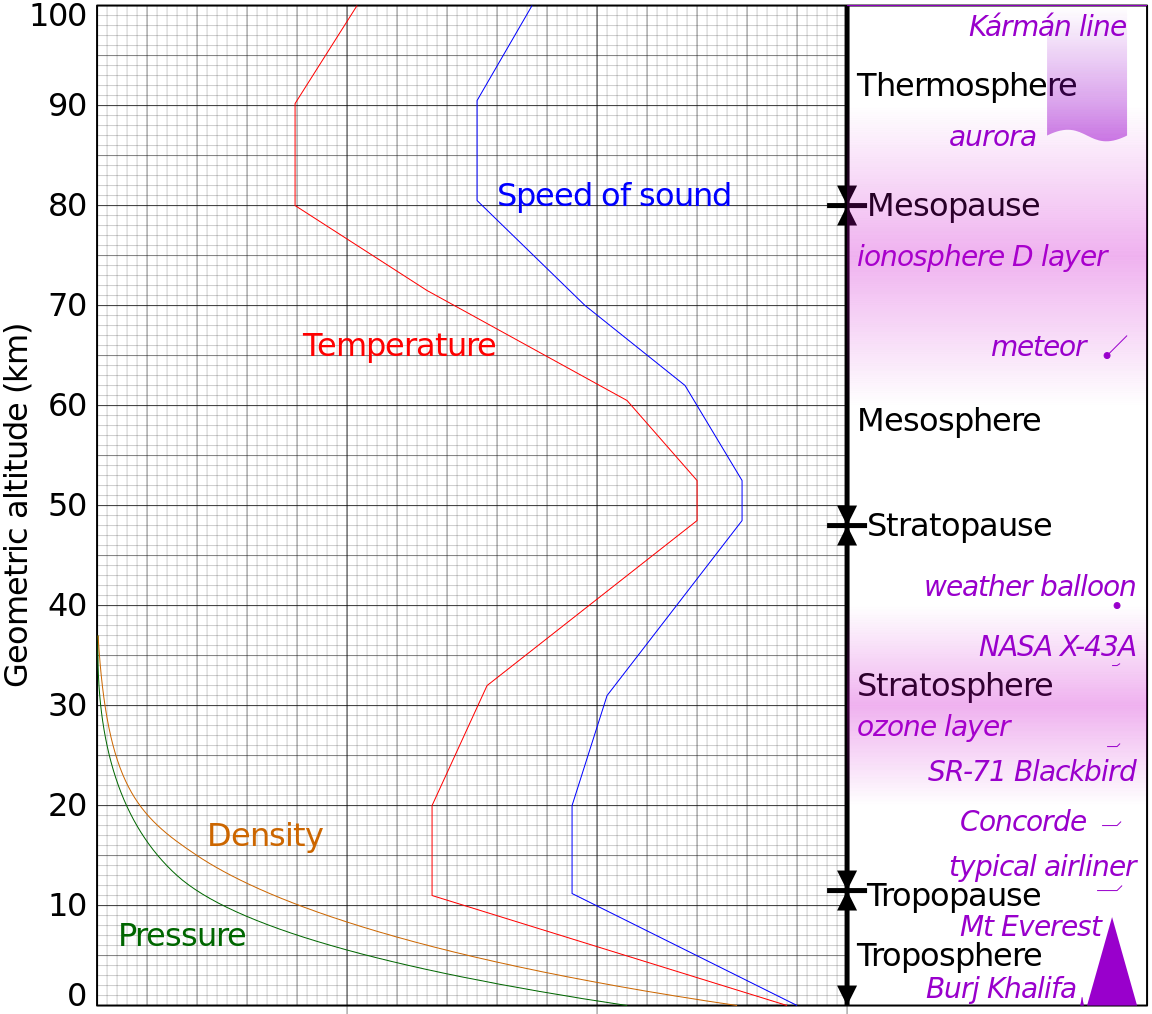
\includegraphics[scale=0.26]{../images/athmosphereProfileCut.png}
    \end{center}    
    
  \end{frame}
  
  \begin{frame}
    \frametitle{Realistische Athmosph"are}
    \framesubtitle{Approximation}
    
    $$n(r) = 1 + \mu \cdot e^{-\sigma (r - r_0)}$$

    $$n_0 = 1.000\,293$$    
    
    $$\mu = n_0 - 1 \approx 2.93 \cdot 10^{-4}$$
    $$\sigma \approx \frac{1}{7} km^{-1}$$
    $$r_0 \approx 6371 km$$
  \end{frame}
  
  \begin{frame}
    \frametitle{Realistische Athmosph"are}
    \framesubtitle{Approximation}
    
    $$n(r) = 1 + \mu \cdot e^{-\sigma (r - r_0)} \qquad n'_r(r) = - \mu \sigma \cdot e^{-\sigma (r - r_0)}$$
    
    $$\mu = 2.93 \cdot 10^{-4} \quad \sigma = \frac{1}{7} km^{-1} \quad r_0 = 6371 km$$

    \begin{center}
      \begin{tikzpicture}
        \begin{axis} [
              axis lines=none, 
              width=6cm, 
              axis equal,
              ticks = none,  
              legend style={at={(1.1,0.5)}, anchor=west, draw=none}, 
              ymin = 1,
              ymax = 21,
              xmin = -10, 
              xmax = 10, 
              view={0}{90}
            ]   
              \draw [draw=none, fill=lGray] (axis cs:0,0) circle (32pt);  
              \shade[even odd rule,ring shading={from llGray at 32pt to white at 52pt}]
                (axis cs:0,0) circle (32pt) circle (52pt);
            
              %a0 = 8.9
              \addplot [mark = none, thick, color=blue] coordinates {
                (0.0000,6.3710)(-0.0854,6.3842)(-0.1711,6.3974)(-0.2573,6.4106)(-0.3440,6.4240)(-0.4513,6.4405)(-0.5595,6.4571)(-0.6685,6.4738)(-0.7785,6.4907)(-0.9645,6.5193)(-1.1536,6.5484)(-1.3463,6.5780)(-1.5429,6.6082)(-1.7439,6.6391)(-1.9498,6.6707)(-2.1611,6.7032)(-2.3782,6.7365)(-2.6019,6.7709)(-2.8327,6.8064)(-3.0713,6.8430)(-3.3186,6.8810)(-3.5754,6.9205)(-3.8428,6.9616)(-4.1217,7.0044)(-4.4134,7.0493)(-4.7193,7.0963)(-5.0409,7.1457)(-5.3801,7.1978)(-5.7388,7.2529)(-6.1193,7.3114)(-6.5245,7.3736)(-6.9573,7.4401)(-7.4215,7.5115)(-7.9214,7.5883)(-8.4622,7.6714)(-9.0499,7.7617)(-9.6920,7.8603)(-10.3975,7.9688)(-11.1776,8.0886)(-12.0459,8.2220)(-13.0203,8.3718)(-14.0236,8.5260)(-15.1558,8.6999)(-16.4456,8.8981)(-17.9312,9.1264)
              };
              \addlegendentry{$\alpha_0 = 81.08^\circ, \: \Delta \alpha \approx 0.174^\circ$};
          
              %a0 = 1
              \addplot [mark = none, thick, color=red] coordinates {
                (0.0000,6.3710)(-0.1286,6.4312)(-0.2598,6.4922)(-0.3938,6.5548)(-0.5306,6.6187)(-0.6706,6.6841)(-0.8140,6.7510)(-0.9610,6.8196)(-1.1119,6.8900)(-1.2669,6.9623)(-1.4264,7.0367)(-1.5907,7.1134)(-1.7601,7.1924)(-1.9351,7.2741)(-2.1160,7.3585)(-2.3033,7.4459)(-2.4975,7.5365)(-2.6992,7.6307)(-2.9091,7.7286)(-3.1276,7.8306)(-3.3557,7.9370)(-3.5941,8.0482)(-3.8438,8.1648)(-4.1058,8.2870)(-4.3812,8.4155)(-4.6714,8.5509)(-4.9778,8.6939)(-5.3021,8.8452)(-5.6462,9.0058)(-6.0122,9.1766)(-6.4027,9.3588)(-6.8205,9.5538)(-7.2690,9.7631)(-7.7521,9.9885)(-8.2744,10.2322)(-8.8413,10.4967)(-9.4593,10.7851)(-10.1362,11.1010)(-10.8815,11.4488)(-11.7068,11.8339)(-12.6265,12.2630)
              };
              \addlegendentry{$\alpha_0 = 64.8^\circ, \: \Delta \alpha \approx 0.059^\circ$};
          
              %a0 = 1
              \addplot [mark = none, thick, color=green] coordinates {
                (0.0000,6.3710)(-0.1251,6.4954)(-0.2552,6.6245)(-0.3908,6.7592)(-0.5323,6.9000)(-0.6804,7.0470)(-0.8354,7.2010)(-0.9982,7.3626)(-1.1693,7.5326)(-1.3496,7.7117)(-1.5400,7.9008)(-1.7415,8.1009)(-1.9553,8.3133)(-2.1827,8.5392)(-2.4252,8.7801)(-2.6847,9.0378)(-2.9631,9.3143)(-3.2629,9.6121)(-3.5868,9.9338)(-3.9381,10.2827)(-4.3208,10.6629)(-4.7397,11.0790)(-5.2004,11.5365)(-5.7099,12.0426)(-6.2770,12.6058)(-6.9124,13.2371)(-7.6297,13.9495)(-8.4465,14.7607)(-9.3862,15.6941)(-10.4798,16.7807)(-11.7675,18.0594)(-13.3093,19.5904)(-15.1917,21.4606)(-16.8948,23.1527)(-18.9317,25.1753)(-21.4179,27.6443)(-24.5257,30.7319)(-27.1015,33.2910)(-30.1918,36.3598)(-33.9782,40.1202)(-38.7332,44.8440)(-42.6155,48.7007)(-47.2755,53.3287)(-52.9886,59.0030)(-60.1683,66.1352)(-66.0243,71.9524)(-73.0544,78.9346)(-81.6748,87.4967)(-92.5103,98.2602)(-101.2007,106.8927)(-111.6034,117.2249)(-124.3122,129.8480)(-140.2120,145.6417)(-146.2182,151.6076)(-152.7488,158.0944)(-159.8760,165.1737)(-167.6860,172.9313)
              };
              \addlegendentry{$\alpha_0 = 45^\circ, \: \Delta \alpha \approx 0.028^\circ$};
          
          \addplot [thick, mark=none, domain=-6.371:6.371, samples=61, forget plot] { sqrt((6.371)^2-x^2)};      
     
        \end{axis}   
      \end{tikzpicture}
    \end{center}        
    
  \end{frame}
  
  \begin{frame}
    \frametitle{Realistische Athmosph"are}
    \framesubtitle{Vergleich}

    %QUELLE:http://jgiesen.de/refract/index.html

    \begin{center}
      \begin{tikzpicture}
	      \begin{axis} [
    	    axis lines=middle,
          xmin = 0,
          xmax = 50,
          ymin = 0,
          ymax = 0.53,
          xlabel={$\alpha_0$},
          ylabel={$\Delta \alpha$},
          width = 9cm,
          height = 7cm,
          xtick = {5, 10, 20, 30, 45},
          xticklabels = {85, 80, 70, 60, 45},
          every axis x label/.style={
    		    at={(ticklabel* cs:1)},
   		      anchor=west,
		      },
		      every axis y label/.style={
 		        at={(ticklabel* cs:1.02)},
  		      anchor=south,
		      },
	      ]
    
    	    \addplot [mark=none, draw=red, thick] coordinates {
    		    (0.0000,0.4830)(0.5000,0.4167)(1.0000,0.3624)(1.5000,0.3182)(2.0000,0.2821)(2.5000,0.2524)(3.0000,0.2277)(3.5000,0.2069)(4.0000,0.1893)(4.5000,0.1743)(5.0000,0.1612)(5.5000,0.1499)(6.0000,0.1399)(6.5000,0.1311)(7.0000,0.1233)(7.5000,0.1163)(8.0000,0.1100)(8.5000,0.1043)(9.0000,0.0991)(9.5000,0.0944)(10.0000,0.0901)(10.5000,0.0862)(11.0000,0.0825)(11.5000,0.0792)(12.0000,0.0760)(12.5000,0.0731)(13.0000,0.0704)(13.5000,0.0679)(14.0000,0.0656)(14.5000,0.0633)(15.0000,0.0612)(15.5000,0.0593)(16.0000,0.0574)(16.5000,0.0557)(17.0000,0.0540)(17.5000,0.0525)(18.0000,0.0510)(18.5000,0.0496)(19.0000,0.0482)(19.5000,0.0469)(20.0000,0.0457)(20.5000,0.0445)(21.0000,0.0434)(21.5000,0.0423)(22.0000,0.0413)(22.5000,0.0403)(23.0000,0.0393)(23.5000,0.0384)(24.0000,0.0376)(24.5000,0.0367)(25.0000,0.0359)(25.5000,0.0351)(26.0000,0.0343)(26.5000,0.0336)(27.0000,0.0329)(27.5000,0.0322)(28.0000,0.0316)(28.5000,0.0309)(29.0000,0.0303)(29.5000,0.0297)(30.0000,0.0291)(30.5000,0.0285)(31.0000,0.0280)(31.5000,0.0274)(32.0000,0.0269)(32.5000,0.0264)(33.0000,0.0259)(33.5000,0.0254)(34.0000,0.0250)(34.5000,0.0245)(35.0000,0.0240)(35.5000,0.0236)(36.0000,0.0232)(36.5000,0.0228)(37.0000,0.0224)(37.5000,0.0220)(38.0000,0.0216)(38.5000,0.0212)(39.0000,0.0208)(39.5000,0.0205)(40.0000,0.0201)(40.5000,0.0197)(41.0000,0.0194)(41.5000,0.0191)(42.0000,0.0187)(42.5000,0.0184)(43.0000,0.0181)(43.5000,0.0178)(44.0000,0.0175)(44.5000,0.0172)(45.0000,0.0169)(45.5000,0.0166)(46.0000,0.0163)(46.5000,0.0160)(47.0000,0.0157)(47.5000,0.0155)(48.0000,0.0152)(48.5000,0.0149)(49.0000,0.0147)(49.5000,0.0144)(50.0000,0.0142)
    	    };
          \draw [dashed] (axis cs:8.92,0) -- (axis cs:8.92,0.174);
          \draw [fill=black] (axis cs:8.92,0.174) circle [radius=0.5mm];
          \draw [dashed] (axis cs:25.2,0) -- (axis cs:25.2,0.059);
          \draw [fill=black] (axis cs:25.2,0.059) circle [radius=0.5mm];
          \draw [dashed] (axis cs:45,0) -- (axis cs:45,0.028);
          \draw [fill=black] (axis cs:45,0.028) circle [radius=0.5mm];
	      \end{axis}
    
      \end{tikzpicture}     
    \end{center}        
    
  \end{frame}
  
  \section{Summary}
  \begin{frame}
    \frametitle{Zusammenfassung}
  \end{frame}
  
\end{document}
